\documentclass[final,2p]{elsarticle}

%% Use the options 1p,twocolumn; 3p; 3p,twocolumn; 5p; or 5p,twocolumn
%% for a journal layout:
%% \documentclass[final,1p,times]{elsarticle}
%% \documentclass[final,1p,times,twocolumn]{elsarticle}
%% \documentclass[final,3p,times]{elsarticle}
%% \documentclass[final,3p,times,twocolumn]{elsarticle}
%% \documentclass[final,5p,times]{elsarticle}
%% \documentclass[final,5p,times,twocolumn]{elsarticle}

\usepackage{amssymb}
\usepackage{amsmath}
%% The amsthm package provides extended theorem environments
%% \usepackage{amsthm}

%% The lineno packages adds line numbers. Start line numbering with
%% \begin{linenumbers}, end it with \end{linenumbers}. Or switch it on
%% for the whole article with \linenumbers after \end{frontmatter}.
%% \usepackage{lineno}
\usepackage{hyperref}
\usepackage{tikz}
\usetikzlibrary{fit,arrows,calc,positioning}

%% natbib.sty is loaded by default. However, natbib options can be
%% provided with \biboptions{...} command. Following options are
%% valid:

%%   round  -  round parentheses are used (default)
%%   square -  square brackets are used   [option]
%%   curly  -  curly braces are used      {option}
%%   angle  -  angle brackets are used    <option>
%%   semicolon  -  multiple citations separated by semi-colon
%%   colon  - same as semicolon, an earlier confusion
%%   comma  -  separated by comma
%%   numbers-  selects numerical citations
%%   super  -  numerical citations as superscripts
%%   sort   -  sorts multiple citations according to order in ref. list
%%   sort&compress   -  like sort, but also compresses numerical citations
%%   compress - compresses without sorting
%%
%% \biboptions{comma,round}

% \biboptions{}


\journal{Udacity}

\begin{document}

\begin{frontmatter}

\title{Capstone Project Proposal}

\author{Martin Pij{\'a}k}

\address{Bratislava, Slovakia}

\begin{abstract}
%% Text of abstract
This is proposal for using Machine Learning methods in futures trading.
\end{abstract}

\begin{keyword}
Machine Learning \sep{Trading} \sep{Udacity} \sep{Nanodegree}
%% keywords here, in the form: keyword \sep keyword

\end{keyword}

\end{frontmatter}

%%
%% Start line numbering here if you want
%%
%% \linenumbers

%% main text
\section{Domain}

In this project we will investigate futures trading on Chicago Mercantile Exchange (CME) markets with Machine Learning methods. The goal is to find the trading strategy mostly based on the price, Commitment of Traders report (COT) and seasonality pattern. We will compare this trading strategy to commonly used investing approaches as returns of Dow Jones Industrial Average or Bonds.

Example of Machine Learning used in futures algorithmic trading.
\begin{itemize}
    \item \href{http://cs229.stanford.edu/proj2014/David\%20Montague,\%20Algorithmic\%20Trading\%20of\%20Futures\%20via\%20Machine\%20Learning.pdf}{Algorithmic Trading of Futures via Machine Learning}
        \begin{itemize}
            \item In this article you can find details about feature engineering, ML-algorithm selection and training
            \item Input vector is 2 years of price and volume data.
        \end{itemize}
    \item \href{https://towardsdatascience.com/https-medium-com-skuttruf-machine-learning-in-finance-algorithmic-trading-on-energy-markets-cb68f7471475}{A Machine Learning framework for Algorithmic trading on Energy markets}
        \begin{itemize}
            \item This article deals with general pipeline setup for trading
        \end{itemize}
\end{itemize}

\section{Datasets and Inputs}
%% \label{S:1}

I will use free data from \href{https://www.quandl.com/}{Quandl}. 

Data range will be from 1st of January 2000. Until current trading day. On average trading year has 252 trading days. This gives us about about 4500 ($252*18 = 4536$) data points (these are composed of multiple values OHLC, COT, date, volume\ldots) over past approximately 18 years.

I will retrieve data through Quandl API and then save resulting dataframe as CSV file.
This way it will be possible to run project without the need to call Quandl APIs.

CME traded commodities below will be used.

\begin{itemize}
\item \href{https://www.cmegroup.com/trading/metals/precious/gold.html}{Gold}
\item \href{https://www.cmegroup.com/trading/agricultural/grain-and-oilseed/corn.html}{Corn}
\item \href{https://www.cmegroup.com/trading/agricultural/softs/coffee.html}{Coffee}
\end{itemize}

I will use COT data joined with trading data (OHLC and volume) daily data.

I might look into other free data sources depending on the results I will get.

\section{Data Analysis Tools}

I plan to use following libraries/frameworks.

\begin{itemize}
    \item \href{https://scikit-learn.org/}{Scikit}
    \item \href{https://keras.io/}{Keras}
    \item \href{https://www.tensorflow.org/}{TensorFlow}
\end{itemize}

\section{Solution Statement}

Main goal is to create trading strategy. I will follow classification approach.

\subsection{Project Design}

Following schema is showing high level project pipeline.
\newline

\tikzstyle{block} = [draw, fill=blue!20, rectangle, 
    minimum height=3em, minimum width=6em]
\tikzstyle{sum} = [draw, fill=blue!20, circle, node distance=1cm]
\tikzstyle{input} = [coordinate]
\tikzstyle{output} = [coordinate]
\tikzstyle{pinstyle} = [pin edge={to-,thin,black}]

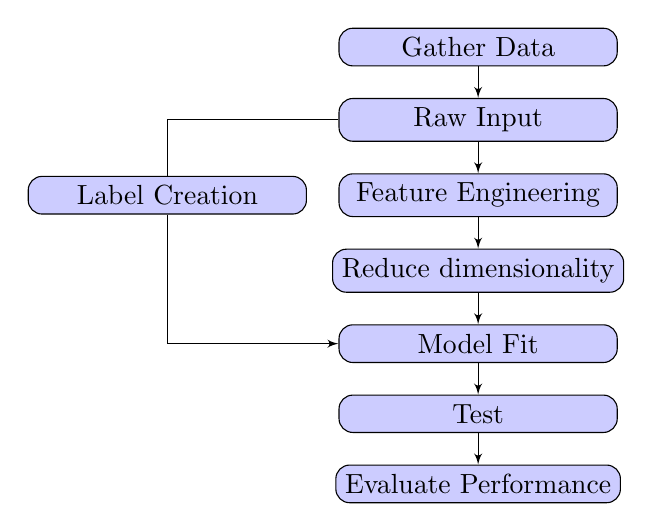
\begin{tikzpicture}[node distance=4mm, >=latex',
 block/.style = {draw, rectangle, minimum height=10mm, minimum width=28mm,align=center},
rblock/.style = {draw, rectangle, rounded corners=0.5em, fill=blue!20,
                 minimum width={width("Reduce dimensionality")+2pt}},
tblock/.style = {draw, trapezium, minimum height=10mm, 
                 trapezium left angle=75, trapezium right angle=105, align=center},
                        ]

    \node [rblock]                      (gd)      {Gather Data};
    \node [rblock, below=of gd]         (input)   {Raw Input};
    \node [rblock, below=of input]      (fe)      {Feature Engineering};
    \node [rblock, below=of fe]         (rd)      {Reduce dimensionality};
    \node [rblock, left=of fe]          (label)   {Label Creation};
    \node [rblock, below=of rd]         (mf)      {Model Fit};
    \node [rblock, below=of mf]         (tst)     {Test};
    \node [rblock, below=of tst]        (perf)    {Evaluate Performance};

    \path[draw,->] (gd)         edge (input)
                   (input)      edge (fe)
                   (fe)         edge (rd)
                   (rd)         edge (mf)
                   (input)      -|   (label)
                   (label)      |-   (mf)
                   (mf)         edge (tst)
                   (tst)        edge (perf)
                    ;
\end{tikzpicture}
\newline
\newline
I will look into commodities that's why I want to capture seasonality.
I plan to use daily data, because of that my trading plan is to hold the position (either long/short) for 1--3 days or until stop loss was hit.

I will investigate different features that have impact on trading.

\begin{itemize}
    \item feature engineering
    \begin{itemize}
        \item PCA (dimensionality of input vector is very high)
        \item COT
        \item price
        \item volume
        \item date (modify to find seasonality)
    \end{itemize}
    \item training
    \begin{itemize}
        \item Random Forest
        \item Neural Network
        \item XGBoost
        \item LightGBM
        \item \ldots
    \end{itemize}
\end{itemize}

How will be stop-loss selected?
\begin{itemize}
    \item fixed
        \begin{itemize}
            \item try different fixed stop-loss values
        \end{itemize}
    \item floating
        \begin{itemize}
            \item based on the volatility of previous days
        \end{itemize}
\end{itemize}

\subsection{Raw Input}
Raw input will have approximately following shape:
\[2 \textup{ years data}\]
\[2*252 \textup{ trading days} = 504\textup{ trading days}\]
\[504\textup{ trading days} * 7 \textup{ (number of features in a day)} = 3528 \textup{ features}\]

\subsection{Feature Engineering}
Reduce dimensionality:
\begin{itemize}
    \item PCA
    \item accumulation
        \begin{itemize}
            \item trading day of month
            \item average
            \item try different min/max of last trading day in relationship to 2years of data
            \item \ldots
        \end{itemize}
\end{itemize}

\subsection{Label Generation}
Labels will be generated as,
% \[
% \begin{align}
\begin{gather}
    fee = 1.5 \\
    t_{treshold} = 30 \\
    v_{volatility} = (\textup{close} - \textup{open})*\delta \textup{ where } \delta \approx 0.95 \\
    %\textup{label} = 
    labels
    \begin{cases}
        | v_{volatility} | > t_{treshold} + fee \implies
        \begin{cases}
            v_{volatility} > 0 \implies 1 \textup{ (long)} \\
            v_{volatility} < 0 \implies -1 \textup{ (short)} \\
        \end{cases}\\
        | v_{volatility} | < t_{treshold} + fee \implies 0 \textup{ (no trade)}
    \end{cases}
% \end{align}
\end{gather}
% \]
$\delta$ constant is used for simulating slippage.
$1.5$ that we are subtracting is a trading fee.
We can see in the label function if volatility is too close to $0$ it will be rounded to $0$ --- meaning don't trade.

Output of model will be classification of input into three categories trade (long/short position) or do not trade.

If we will look into longer trading than one day. Labels can be constructed in the similar way as above. But we will have to consider stop-loss value. We might have to end the trade sooner than we wanted.

\section{Benchmark Model}

I will use three benchmarks for my model

\begin{itemize}
    \item fixed percentage (bank/bond deposit comparison)
    \item Dow Jones Industrial Average performance
    \item mean reversal trading on given commodity markets
\end{itemize}

\section{Evaluation Metrics}

For simulation purpose I will calculate account gains with account size of $10,000\$$.

Trained models will be evaluated compared to Benchmark Models. Based on the one of trading signals $(-1,0,1)$ (output of huge input vector) gain or loss will be calculated --- taking into account stop-loss.
I plan to use 8 years for training and 2 years of data for model evaluation. I plan to trade only one contract regardless of the account size over time.

\end{document}
